\documentclass[12pt,a4paper]{article}
\usepackage[utf8]{inputenc}
\usepackage{graphicx}
\usepackage{tikz}
\usetikzlibrary{fit}
\usepackage{lmodern}
\usepackage{sectsty}


\sectionfont{\color{cyan}}

\begin{document}
   \begin{titlepage}
      {\fontfamily{lmss}\selectfont
      	\centering
      	
\includegraphics[width=0.30\textwidth]{logo.png}\par\vspace{1cm}
      	{\LARGE Capstone Project Demo 1 \par}
      	\vspace{0.25cm}
      	{\huge\bfseries \color{cyan}System Requirements and Design Document\par}
      	\vspace{1cm}
      	{\Large\textit{by} Brute Force\par}
         \vspace{0.25cm}
         \begin{tikzpicture}
            \node [inner sep=0pt,,outer sep=0pt,clip,rounded corners=0.5cm] (pict) at (0,0) {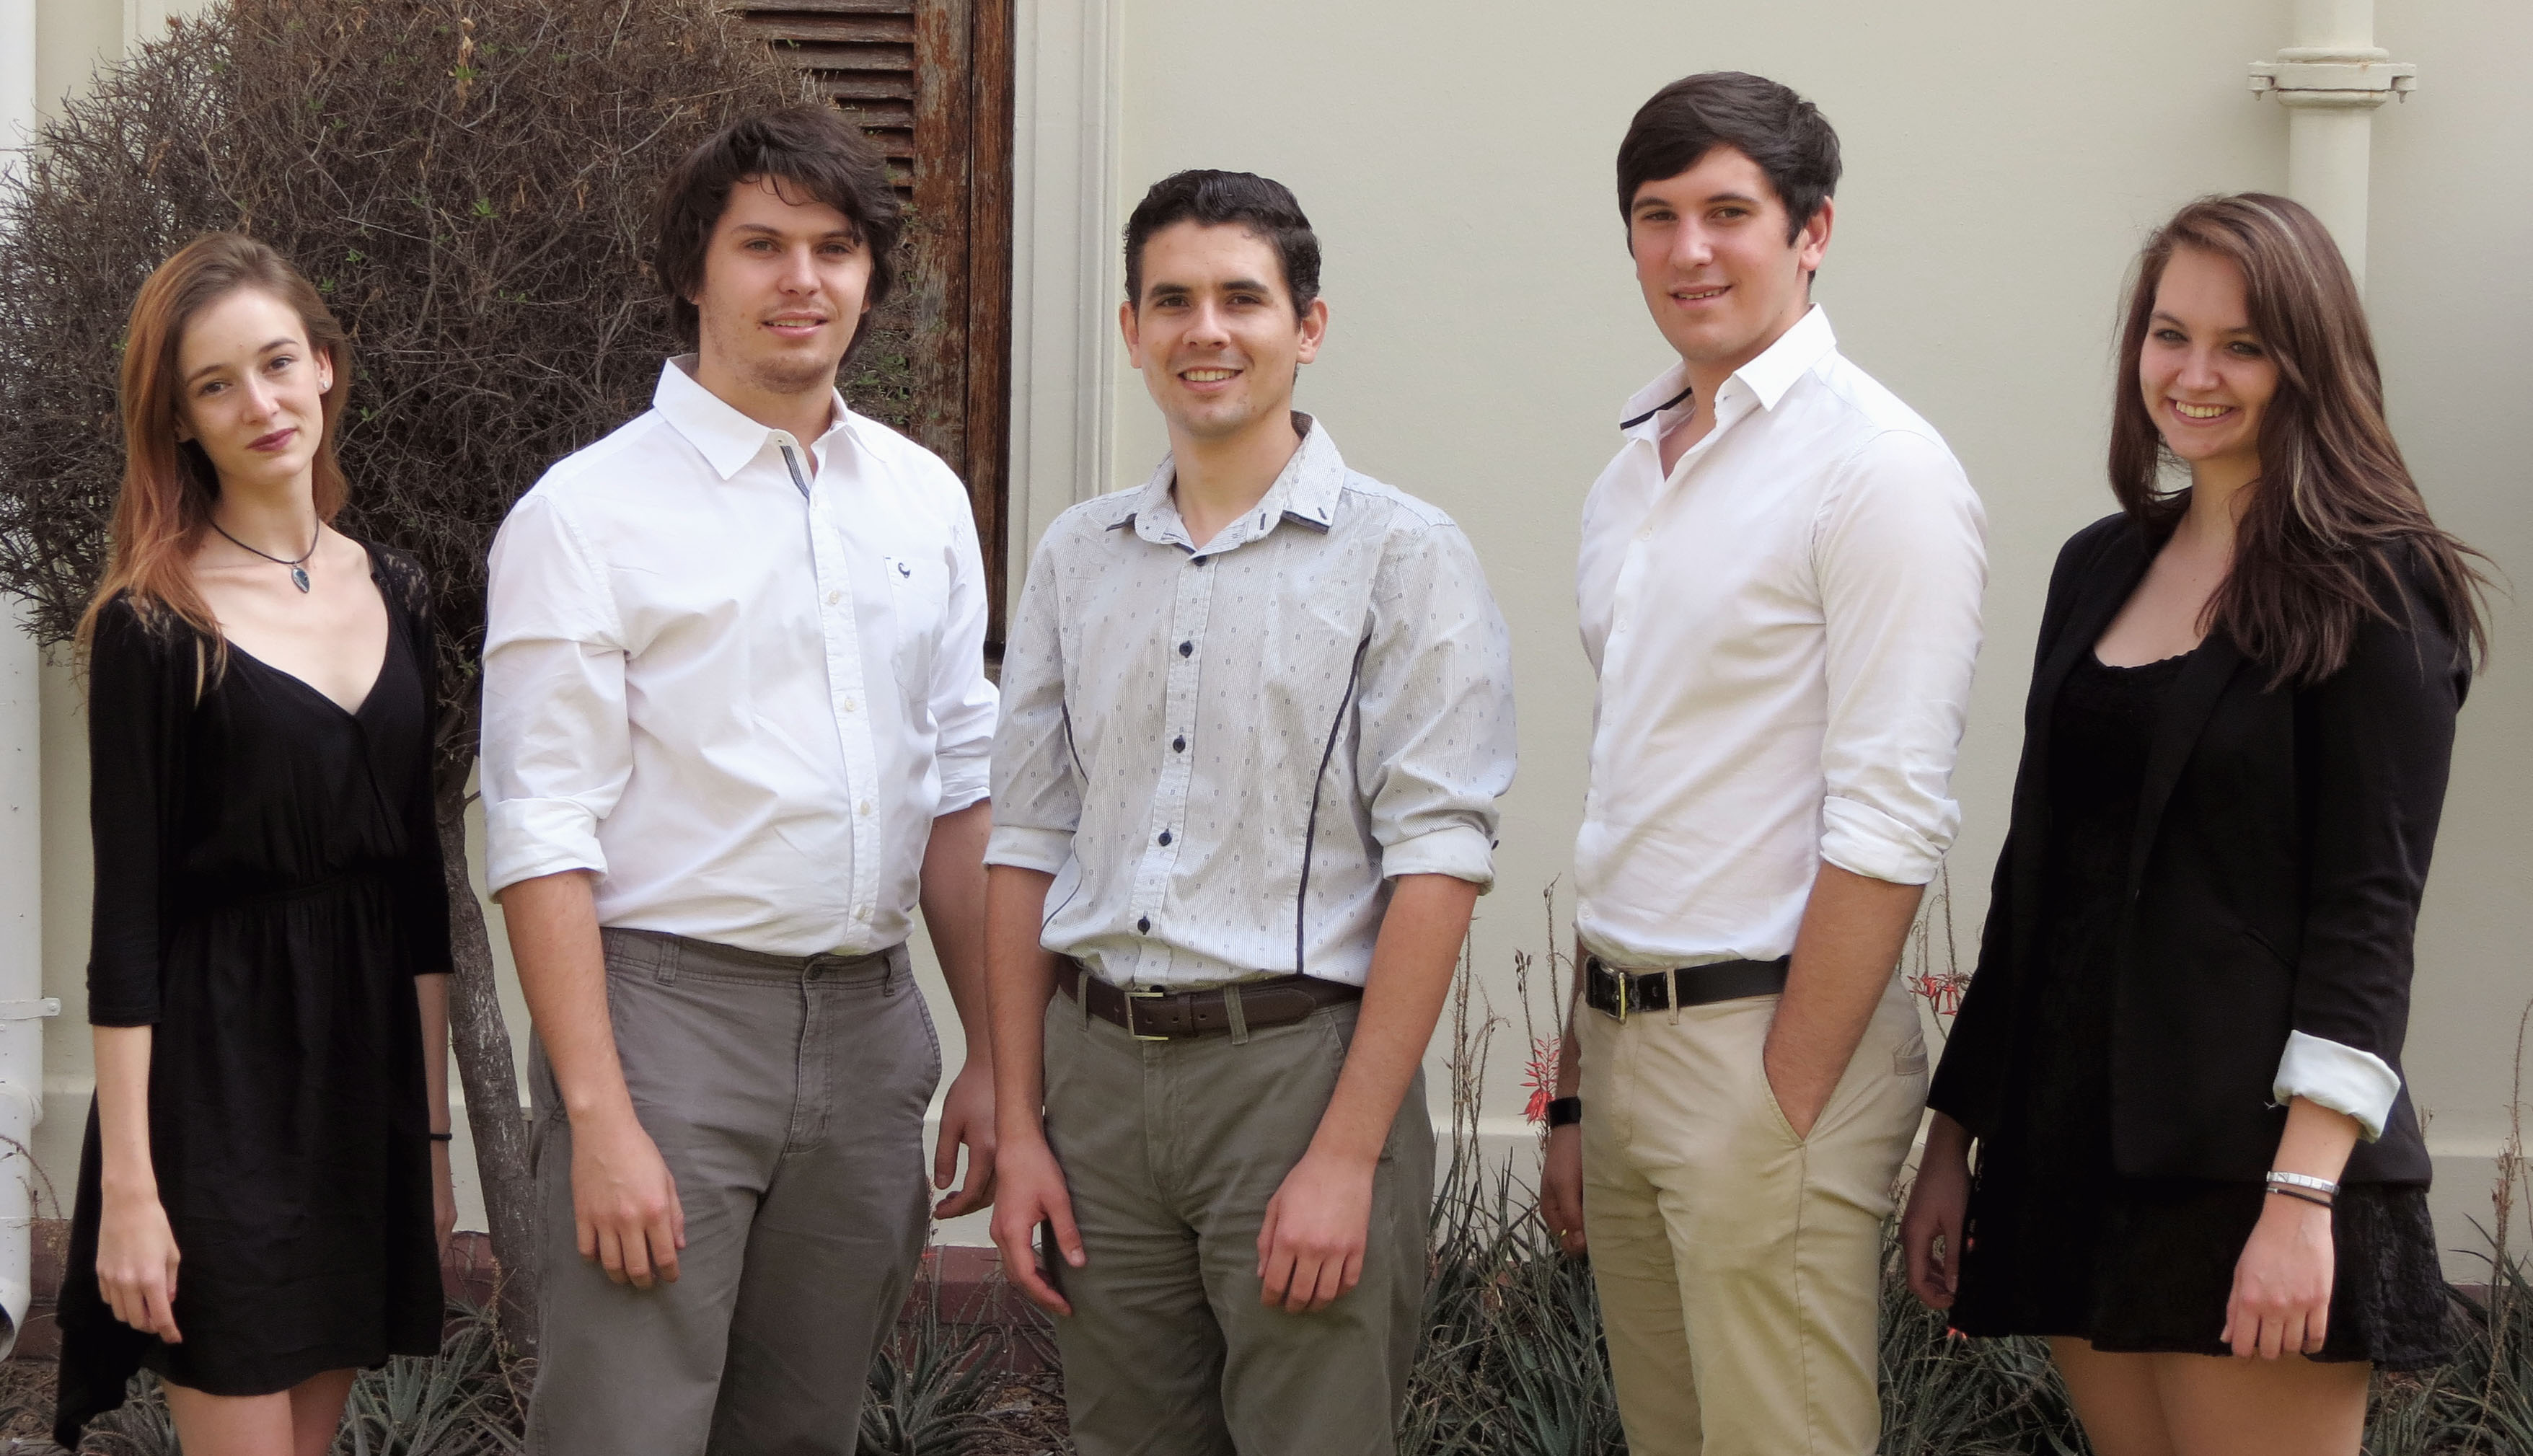
\includegraphics[width=0.9\textwidth]{team.jpg}};
            \node[fit=(pict),rounded corners=.55cm,inner sep=2pt]{};
         \end{tikzpicture}

         \par\vspace{1cm}
         \date{}
         \author{}
         \title{}
         \centering
         \textbf{Authors:}\\
         Mia Gerber\\
         Matthew Perry\\
         Wanrick Willemse\\
         Duart Breedt\\
         Linda Potgieter\\
      }
   \end{titlepage}
   \maketitle
   \tableofcontents
   \newpage

   \section{Introduction}
   	\subsection{Purpose}
		\paragraph{Application for splitting a restaurant bill between friends.}
		The application will be used as a utility in a social context to decrease the time it takes to work out how much everyone needs to contribute to a shared bill.

   	\subsection{Scope}
   	This project will essentially be divided into two phases, the first of which focuses heavily on user experience and the second accuracy.
		\paragraph{Phase One:}
		A multi-platform mobile application that users can send a photo of a bill to and receive an interactive interface generated from the data contained within that photo that they can then use to work out correct totals.
		\paragraph{Phase Two:}
		An artificial intelligence agent that has been trained to recognise text in a photo in a very specific way will be the backend mechanism that can be given any photo and will return a JSON object with the structure of that photo that can be parsed to create the interface in phase one.

   	\subsection{Overview}
The goal of this document is to define a clear project scope that will be used to contain and guide coming deliverables as well as give clarity as to how our application will function as a system built up out of well-defined components.

   \section{Overall Description}
   	\subsection{System Interfaces}
   		%Wanrick
		The Split Bill system has no existing external interfaces. The system will consist of a webbased OCR system that detects and identifies a receipt format. The webbased system interfaces with a user's mobile device.
   	\subsection{User Interfaces}
   		%Mia
   	\subsection{Hardware Interfaces}
   		%Matthew
   		The Split Bill application will make use of of the camera on the device. The data modules (WiFi and mobile data) will be used for connection to the server over the internet.
   	\subsection{Software Interfaces}
		%Matthew
   		% UML diagrams will go here
   	\subsection{Product Functions}
		%Wanrick
		Using the mobile interface, a user will be able to take a photo of a restaurant receipt. The mobile device will position and crop the image to only include the restaurant name, items and amounts listed and the totals. On succesful upload a user session is created. The session ID is returned to the initiating user's mobile device. The mobile app then provides a session ID in text format that can be shared with other users using a QR barcode or NFC.\\
		The image is uploaded to a webserver where OCR is used to extract the information on the receipt. The information extracted from the image will be analyzed and an AI will determine the closest matching receipt format. The information from the image along with the determined format will be used to create a JSON object that is returned to all the users connected to the session.\\
		Each user will be able to set a nickname and avatar colour to identify each user. A user will be able to select items from the receipt that is then regarded as claimed, blocking the item for every other user in the session. As a user claims an item, his total will be updated. Once all the items have been claimed, a user can choose a tip percentage. The user's total contribution will be displayed to the user.
   		% Use cases could possibly be sensible here
	\subsection{User Characteristics}
   		% actor-system modelling
		Our application is being marketed as a "utility" and as such we won't be targeting a specific user, we want to appeal to as many people as possible because the type of person who visits a restaurant with friends is almost every person imaginable. With that said we will however assume our users to be literate in mobile technologies. A basic understanding of touch screen gestures and navigation between different screens will be assumed. We are making HCI (Human Computer Interaction) a major focus during development of our GUI and as such the aim is simplicity and usability without losing aesthetic appeal.

   	\subsection{Assumptions and Dependencies}
		 \begin{itemize}
	\item All team members are available and have the necessary skills and knowledge to collaborate and complete the project. 
Set deadlines and milestones area achievable and project can be finished by the October deadline.   
\item There will be an external server provided to which data can be sent from applications that have Internet connection. 
\item The application will be open source. This means open source libraries will be used for most of the applications components such as including more complex aspects such as OCR and peer to peer connectivity. 
\item OCR technology will be able to convert images uploaded to the server to a standardized file format.
\item The application will have to be able to operate on all available mobile operating systems. 
\end{itemize}
   \section{Specific Requirements}
	\subsection{External Interface Requirements}
		%Matthew
		\subsection{Hardware Interface}
		The Split Bill system will be designed to be run off of a smart phone. The system will make use of the smart phone's camera in order to take a picture of the bill for processing.
		\subsection{Software Interface}
		The user will interact with the application through a touch screen interface on the device. 
		\subsection{Communications Interface}
		The WiFi module, or the mobile network module will be used to establish a connection over the internet to the central server. Through this server, the user will be able to communicate with other users and split the bill with them.
		\subsection{User Interface}
		The user interface will be a full screen application that will be designed following HCI protocols to ensure that the optimal user interface that will serve all the functional requirements.
	\subsection{Functional Requirements}
		\begin{enumerate}
				\item The system must be able to recognise text on a bill.
				\item The system must be able to correctly categorise the different "columns" of text into discrete structures that represent different information semantically (e.g. an item of food is not interpreted as a numeric amount)
				\item The system should consciously check whether it has correctly interpreted the bill and if it did not ask the user either for a higher quality photo or as a last resort give an error message.
				\item The system should return all information gleaned from the OCR process as a JSON object of which the structure is known to the component that will be receiving the object.
			\end{enumerate}

			\begin{enumerate}
				\item The user interface provides a facility for both taking a photo and sending it to the server.
				\item The user interface provides a facility for starting a new session which will return a temporary session code which is shared with users who also have the application around the table.
				\item The user interface which is generated after interpretation of the bill (after the associated JSON object has been received) contains a  facility for choosing items to pay for and generates a running total as the user decides.
				\item All user that were added to the current session will receive the exact same interface and as such will be able to see which items are still available to be paid for and which are no longer available. (Asynchronous calls to the server will facilitate updating of the user interface)
			\end{enumerate}

	\subsection{Performance Requirements}
		Since the application is user based, performance is of utmost importance. The application should be very responsive and be able to process user information and requests in an appropriate amount of time to ensure the user has a pleasant experience. Performance requirements will focus on response time, completion time, efficiency and speed up, without compromising on functionality and effectiveness. 
	\subsection{Design Constraints}

		\begin{itemize}
			\item Even though we will not be persisting any image data for longer than necessary the size of images being sent to the server is a constraint we will need to be conscious of, possible solutions will be cropping or simply reducing image quality by changing the image to only use black and white or a degree of grayscaling.
			\item The experience of the development team might influence the degree to which the artificial intelligence portion of this project comes to fruition.
			\item The possibility of getting the application to still be functional without internet access can become a design constraint later in development.
		\end{itemize}

	\subsection{Software System Attributes}
   		%Matthew
\end{document}
